In order to formally develop the concepts of intrinsic and extrinsic homotopy for language encoders, we first need some basic mathematical notions.
The aim of this chapter is to provide a theoretical framework in which encoders can be compared with respect to their similarity using transformations. 
To this end, we first introduce \emph{hemi-metric spaces} in Section ~\ref{HMS} , which enable an asymmetric distance function between language encoders.
This structure allows us to measure similarities without necessarily requiring symmetry or the triangle inequality, properties that are often not given in practical comparison scenarios.
Based on this, we define the norms and distances in Section ~\ref{ND} in the space of language encoders.
These measures are crucial for mathematically quantifying differences between encoders and analyzing transformations. %Der Copilot schlägt hier immer analyzing vor und die Rechtschreibprüfung sagt immer analysing
A central concept, the so-called \emph{Specialisation Quasi-Ordering}, which is a special form of preordering derived from the hemi-metric structure, is presented in Section ~\ref{sec:sqp}.
It describes whether one encoder can be completely transformed into another one.
Finally, we motivate \emph{homotopy} in Section ~\ref{UHtMS} to measure similarity.


\section{Hemi-Metric Spaces}\label{HMS}
In the following, we will use the definition of metrices and a hemi-metric as tom Dieck \cite{dieck_mengentheoretische_top} defined.
Further, we consider Metric Spaces $(X,d)$, that is, a set $X$ and a metric $d$ operation on $X$.
A metric on a set $X$ is a mapping $d:X\times X \rightarrow [0,\infty[$ that satisfies the known axioms:
\begin{itemize}
    \item [M1] $d(x,y) > 0$ and $d(x,y) = 0 \Leftrightarrow x=y$
    \item [M2] $d(x,y)=d(y,x) \quad \forall x,y\in X$
    \item [M3] $d(x,z) \leq d(x,y) + d(y,z) \quad \forall x,y,z \in X$
\end{itemize}

If there is a map $d:X\rightarrow \overline{\mathbb{R}}_+$, that means that the metric can be equal to $\infty$ and we denote it as an \textbf{extended metric}.
A \emph{hemi-metric} or \emph{Lawvere metric}~\cite{lawvere_metric_1973} is a generalized distance function that relaxes the symmetry requirement of a metric.

\begin{definition}[Hemi-metric / Lawvere metric]\label{def:hemi_metric}
Let \( X \) be a set.  
A function \( d \colon X \times X \to \overline{\mathbb{R}}_+ \) is called a \emph{hemi-metric} (or \emph{Lawvere metric}~\cite{lawvere_metric_1973}) if it satisfies the following two axioms:
\begin{itemize}
    \item [H1] \( d(x, x) = 0 \) for all \( x \in X \),
    \item [H2] \( d(x, z) \le d(x, y) + d(y, z) \) for all \( x, y, z \in X \).
\end{itemize}
Note that symmetry is not required, i.e., it may hold that \( d(x, y) \ne d(y, x) \).  
If the codomain includes \( \infty \), we call \( d \) an \emph{extended hemi-metric}.
\end{definition}



This relaxation allows us to define an asymmetric notion of distance between representations.
In particular, we can formalize how far a language encoder \( h \) is from the set of all possible transformations of another encoder \( g \).
To this end, the hemi-metric is lifted from individual elements \( x \in X \) to subsets of \( X \).
\begin{definition}[Hausdorff-Hoare map]\label{def:hausdorffHoareMap}
Let $(X,d)$ be a hemi-metric space, and let $E, E' \subset X$ be non-empty subsets.  
The \emph{Hausdorff-Hoare map} is the function
\[
d^{\mathcal{H}}(E, E') := \sup_{x \in E} \inf_{y \in E'} d(x, y),
\]
that defines a hemi-metric on $\mathcal{P}(X) \setminus \{\emptyset\}$.
\end{definition}

If $E$ is considered as a singleton set $\{x\}$, we will write $d^\mathcal{H}(x,E')$ instead of $d^\mathcal{H}(\{x\},E'):=\inf\limits_{g\in E'}d(x,y)$

%Further, if we want to define a hemi-metric on a set $X$ by embedding $X$ into the power set of a second space $Y$ where a hemi-metric exists.
%The Hausdorff-Hoare map based on the hemi-metric of $Y$ can be used after $X$ is embedded to define a hemi-metric in $X$ through the images of $x \in X$.
If a set \( X \) does not itself carry a hemi-metric, but can be embedded into the power set of a second space \( Y \) that does, we can induce a hemi-metric on \( X \) via this embedding.  
Specifically, let \( \varphi: X \to \mathcal{P}(Y) \setminus \{\emptyset\} \) be an embedding of \( X \) into non-empty subsets of \( Y \).  
Then a hemi-metric on \( X \) can be defined by
\[
d_X(x, x') := d^\mathcal{H}(\varphi(x), \varphi(x')),
\]
where \( d^\mathcal{H} \) is the Hausdorff–Hoare map induced by the hemi-metric on \( Y \).


\section{Norm and Distances}
\label{ND}
%To follow the hemi-metric recipe, it is required, to define a hemi-metric on the individual elements.
%Let \( V \) be a finite-dimensional \( \mathbb{R} \)-vector space, equipped with a norm \( |\cdot|_V \). Since all norms on finite-dimensional spaces are equivalent, we fix one such norm for the remainder. 

%We consider the space of encoder functions \( \mathcal{E}_V \subset \{ h : \Sigma^* \to V \} \), equipped with the norm:
%\[
%\|h\|_\infty := \sup_{y \in \Sigma^*} |h(y)|_V,
%\quad \text{and corresponding metric} \quad
%d_\infty(h, g) := \|h - g\|_\infty.
%\]
%Assuming that \( \mathcal{E}_V \) is closed under this norm, the space \( (\mathcal{E}_V, d_\infty) \) is a complete metric space. This follows from the completeness of \( V \) and the definition of the supremum norm on function spaces.


As is well known, every norm on a real vector space induces a metric via \( d(x, y) := \|x - y\| \).  
Since all norms on a finite-dimensional \(\mathbb{R}\)-vector space \(V\) are equivalent \cite{lang_algebra_2002}, we will work with a fixed norm \(|\cdot|_V\) on \(V\) in the following.


%As all norms in the $\mathbb{R}$-vector space $V$ are equivalent, the norm $|\cdot|_V$ on $V$ will be considered in the following.

We further define the extended norm
\[
\|h\|_\infty := \sup_{y \in \Sigma^*} |h(y)|_V,
\]
and the induced metric
\[
d_\infty(h, g) := \|h - g\|_\infty
\]

on the space \(\mathcal{E}_V\), which consists of all functions \(h : \Sigma^* \to V\) with finite \(\|\cdot\|_\infty\)-norm.
%A metric space where every Cauchy sequence converges to a point within the space. 
%That is given by the fact that $|\cdot|_V$ is a norm and the completeness of $V$.

Equipped with this metric, \((\mathcal{E}_V, d_\infty)\) forms a complete metric space, meaning that every Cauchy sequence in \(\mathcal{E}_V\) converges to a limit within the space.  
This follows from the fact that \(V\) is a finite-dimensional normed space and hence complete.
This property will later be used to argue the existence of certain infima in \(\mathcal{E}_V\).



For the subordinate matrix norm we write $\|\cdot\|_V: GL(V) \rightarrow \mathbb{R}_+$, where $GL(V)$ denotes the set of invertible $D\times D $ matrices.
It is defined as \[\|W\|_V=\sup_{v\in V\setminus \{0\}}\frac{|W v|_V}{|v|_V}.\]
We consider $V$ as an affine space and set $\text{Aff}(V)$ for the group of affine transformations of $V$, by abuse of language, if we forget about the special role that the zero vector has.

A map $v\mapsto Wv +b$ is called an affine transformation $\psi$ on $V$ for $W\in GL(V)$ invertible and $b \in V$.
The transformation consists of a linear part $\psi_{lin}:=W$ and a translation part $\psi_t:v\mapsto v+b$.
Further, $\mathcal{T}\subset \text{Aff}(V)$ denotes the subgroup of translation.
There is also a natural left action on $\text{Aff}(V)$ on $\mathcal{E}_V$.
I.e. $\text{Aff}(V)\times \mathcal{E}_V\rightarrow \mathcal{E}_V, h \mapsto \psi\circ h$, such that there exists an identity element $e$ on $\text{Aff}(V)$, where $e\cdot h = h \quad \forall h\in \mathcal{E}_V$ and $\psi_1\cdot(\psi_2\cdot h)=(\psi_1\psi_2)\cdot h \quad \forall \psi_1,\psi_2 \in \text{Aff}(V)\ \text{ and } h \in \mathcal{E}_V$.

\section{Specialization Quasi-ordering and Pre-ordering}\label{sec:sqp}
In this section, we formalize the notion of specialization quasi-ordering and show that it induces a preorder.
This structure will be used to define various homotopies on language encoders in later sections.
We follow the exposition of Goubault-Larrecq in \cite{goubault-larrecq_non-hausdorff_nodate}.

We begin with a brief reminder of the concept of a topological space.
A \emph{topological space} is a set $X$ equipped with a collection of subsets, called \emph{open sets}, that satisfies the following properties:
\begin{itemize}
\item The empty set $\emptyset$ and the full set $X$ are open.
\item Arbitrary unions of open sets are open.
\item Finite intersections of open sets are open.
\end{itemize}
This collection of open sets defines the topology on $X$.

\begin{definition}[Base]
        Let $X$ be a topological space, and $\mathcal{B}$ be a family of open subsets of $X$.
        If every open set is a union of elements of $\mathcal{B}$, $\mathcal{B}$ is a \emph{base} of the topology. 
\end{definition}

\begin{lemma}[Characterization of a Basis]\label{lem:basis_characterization}
A family \(\mathcal{B}\) of subsets of a topological space \(X\) is a basis of the topology if and only if for every open set \(U \subseteq X\) and every point \(x \in U\), there exists an element \(V \in \mathcal{B}\) such that \(x \in V \subseteq U\).
\end{lemma}

\begin{proof}
Let \(U\) be open and \(x \in U\). 
By assumption, there exists \(V_x \in \mathcal{B}\) with \(x \in V_x \subseteq U\).  
Using the Axiom of Choice, pick such a \(V_x\) for each \(x \in U\), and write \(U = \bigcup\limits_{x \in U} V_x\).

Suppose \(\mathcal{B}\) is a basis, and let \(U = \bigcup\limits_{i \in I} V_i\) with \(V_i \in \mathcal{B}\). 
For any \(x \in U\), there exists some \(i \in I\) such that \(x \in V_i\). Let \(V := V_i\), then \(x \in V \subseteq U\).
\end{proof}


\begin{definition}[Specialization Quasi-ordering]\label{def:quasi-ordering}
Let $X$ be a topological space. 
The specialization quasi-ordering on $X$ is defined by:
\[
x \gtrsim y \quad \text{if and only if} \quad \text{every open set containing } x \text{ also contains } y.
\]
\end{definition}

This quasi-ordering induces a preorder on $X$, as stated in the following lemma.


\begin{lemma}[Preorder]\label{lemma:preorder}
The specialization quasi-ordering is a preorder; that is, it is reflexive and transitive.
\end{lemma}


\begin{proof}
Let $\gtrsim$ denote the specialization quasi-ordering.

\textbf{Reflexivity:} For any $x \in X$, every open set containing $x$ trivially contains $x$ itself, so $x \gtrsim x$.

\textbf{Transitivity:} Suppose $x \gtrsim y$ and $y \gtrsim z$. Let $U$ be an open set containing $x$. Then, by definition of $\gtrsim$, $y \in U$, and hence $z \in U$. Therefore, $x \gtrsim z$.
\end{proof}


Now consider a hemi-metric $d$ on a set $X$. We define open balls by
\[
B(x, \varepsilon) := \{ z \in X \mid d(x, z) < \varepsilon \},
\]
where $x \in X$ is the center and $\varepsilon \in \mathbb{R}^+$ the radius.
The topology generated by such open balls is referred to as the \emph{open ball topology}.

\begin{lemma}[Open Balls Form a Base]\label{lemma:open_balls_form_base}
Let $(X, d)$ be a hemi-metric space.
Then, for every open set $U$ containing $x \in U \subset X$, there exists $\varepsilon > 0$ such that
\[
B(x, \varepsilon) \subset U.
\]
\end{lemma}

\begin{proof}
Let $U$ be an open set containing $x \in X$. By the definition of the topology induced by $d$, there exists a finite collection of open balls $B(x_i, \varepsilon_i)$, $1 \leq i \leq n$, such that
\[
x \in \bigcap_{i=1}^n B(x_i, \varepsilon_i)\subset U.
\]
We show that there exists an open ball $B(x, \varepsilon)$ centered at $x$ such that
\[
B(x, \varepsilon) \subseteq \bigcap_{i=1}^n B(x_i, \varepsilon_i)\subset U.
\]

Define
\[
\varepsilon := \min_{1 \leq i \leq n} \left( \varepsilon_i - d(x_i, x) \right).
\]
Since $x \in B(x_i, \varepsilon_i)$ for each $i$, we have $d(x_i, x) < \varepsilon_i$, and thus $\varepsilon > 0$.

Now take any $y \in B(x, \varepsilon)$, i.e., $d(x, y) < \varepsilon$.
By the (possibly asymmetric) triangle inequality for hemi-metrics, we get
\[
d(x_i, y) \leq d(x_i, x) + d(x, y) < d(x_i, x) + \varepsilon \leq \varepsilon_i,
\]
so $y \in B(x_i, \varepsilon_i)$ for all $i$. Hence,
\[
B(x, \varepsilon) \subseteq \bigcap_{i=1}^n B(x_i, \varepsilon_i) \subset U.
\]

Therefore, for every open set $U$ and every point $x \in U$, there exists an open ball $B(x, \varepsilon) \subseteq U$. By Lemma~\ref{lem:basis_characterization}, the collection of open balls forms a basis for the open ball topology.
%\noindent\textit{Recall:} A family \( \mathcal{B} \) of subsets of a topological space \( X \) is a base of the topology if and only if, for every open set \( U \subseteq X \) and every point \( x \in U \), there exists a set \( V \in \mathcal{B} \) such that \( x \in V \subseteq U \).
\end{proof}



\section{Using Homotopy to Measure Similarity}\label{UHtMS}

Within this section, we follow the notion of homotopy as introduced by Knudson \cite{knudson_algtop}. 
Let \( X \) and \( Y \) be topological spaces.

A function \( f: X \rightarrow Y \) is called \emph{continuous} if the preimage \( f^{-1}(V) \subseteq X \) is open for every open set \( V \subseteq Y \).

Let $A$ be a subspace of $X$, then $(X,A)$ is called a pair. 
Further, if we have a continuous map $f:X \rightarrow Y$ that maps a subspace $A\subset X $ into the subspace $B \subset Y$, we write $f: (X,A) \rightarrow (Y,B)$.


\begin{definition}[Homotopy]
	Let \( f, g \colon (X,A) \rightarrow (Y,B) \) be two continuous maps that agree on \( A \subseteq X \).  
	A continuous map
	\[
	H \colon X \times I \rightarrow Y, \quad \text{with } I = [0,1],
	\]
	is called a \emph{homotopy from \( f \) to \( g \) relative to \( A \)} if the following properties hold:
	\begin{enumerate}
		\item \( H(x,0) = f(x) \) for all \( x \in X \),
		\item \( H(x,1) = g(x) \) for all \( x \in X \),
		\item \( H(a,t) = f(a) \) for all \( a \in A \) and \( t \in [0,1] \).
	\end{enumerate}
	In this case, we write \( f \simeq g \) rel \( A \).  
	The interval \( I = [0,1] \) is chosen without loss of generality, as any closed interval can be rescaled to this standard domain.
\end{definition}

If there exists a homotopy between two continuous maps \( f, g \colon X \rightarrow Y \), then \( f \) and \( g \) are said to be \textbf{homotopic}.

A homotopy \( H \) can be interpreted in two equivalent ways:
\begin{itemize}
	\item For each point \( x \in X \), the map \( t \mapsto H(x,t) \) defines a path in \( Y \) from \( f(x) \) to \( g(x) \), which depends continuously on \( x \).
	\item For each \( t \in [0,1] \), the map \( x \mapsto H(x,t) \) defines a continuous map \( H_t \colon X \rightarrow Y \), and the family \( (H_t)_{t \in [0,1]} \) varies continuously with \( t \).
\end{itemize}

In this sense, a homotopy is a \textbf{continuous deformation} of \( f \) into \( g \).



Consider the map  $F : \mathbb{R} \times [0, 1] \to \mathbb{R} $
given by 
$ F(x, t) = x^3 + tx + 1. $
Since this is continuous, it is a homotopy from 
$ f_{-1}(x) = x^3 - x + 1 $
and
$ f_1(x) = x^3 + x + 1$ \cite{knudson_algtop}.
\begin{center}
    \begin{figure}[H]
        \centering
        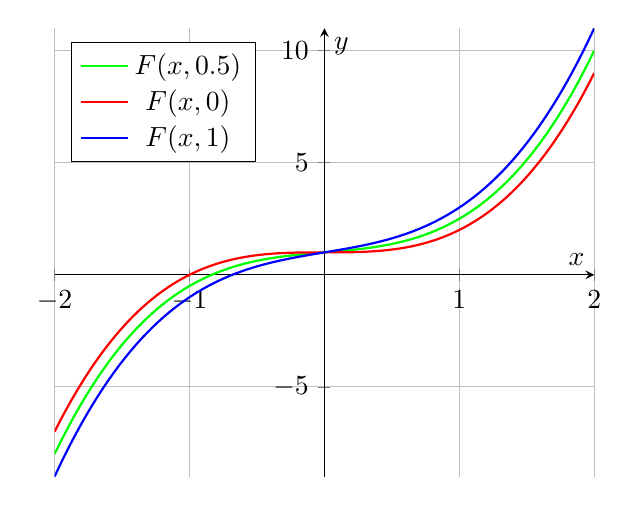
\begin{tikzpicture}
            \begin{axis}[domain=-2:2, samples=100, axis lines=center, xlabel={$x$}, ylabel={$y$}, grid=major, legend pos=north west]
                \addplot[green, thick] {x^3 + 0.5*x + 1};
                \addlegendentry{$F(x, 0.5)$}
                \addplot[red, thick] {x^3 + 1};
                \addlegendentry{$F(x, 0)$}
                \addplot[blue, thick] {x^3 + x + 1};
                \addlegendentry{$F(x, 1)$}
            \end{axis}
        \end{tikzpicture}
        \caption{Plot of the homotopy function $F(x,t) = x^3 + tx + 1$ for different values of $t$.}
        \label{fig:homotopy_plot}
    \end{figure}
\end{center}

Let \( \mathcal{E}_V \) denote a set of encoders, i.e., functions from a set \( X \) into a vector space \( V \).  
Define \( \mathcal{C}_{V,W} := \{ \varphi \colon V \to W \mid \varphi \text{ is continuous} \} \).  
Let \( S \subseteq \mathcal{C}_{V,W} \) be a specified class of admissible transformations between representation spaces, such as the set of all continuous, smooth, or affine maps.



Two encoders \( f, g \in \mathcal{E}_V \) are called \emph{\(S\)-homotopic} if there exists a transformation \( \psi \in S\) such that \( f \) can be approximated by \( \psi \circ g \).

We refer to this notion as \emph{\(S\)-homotopy}, and study it as a framework to compare encoders via transformations in \(S\).  
Accordingly, we define the set
\[
E_h := \left\{ f \in \mathcal{E}_V \mid \exists\, \psi \in S\text{ such that } f \approx \psi \circ h \right\},
\]
which collects all encoders to which \( h \) can be transformed via \(S\)-mappings.

A special case is obtained by taking \(S= \mathrm{Aff}(V) \), the set of affine maps on \( V \), which corresponds to the affine encoder framework studied in the work of Chan et al. \cite{chang_clust_met_space}.
